\section{Tests}
\begin{enumerate}
\item Introduction to the section. What do we want and why. First we want to test A and the X. At last we want to test the complete system.
\item Introduce how we will compare the tests and how we measure the quality -- Mean Squared Error (MSE).
\item Subsection with the error measure
\item Subsection with a introduction to the data sets -- AR and Toy Example data sets.
\item Subsection with the performing of tests
	\begin{itemize}
	\item Talk about the choice for a initial A in the Cov-DL when D is under-complete. Random uniform distribution? or a Gaussian distribution. Show the errors of the real A and estimated A.
	\item With the choice for A we now tests the choice for the number of segmentation in Cov-DL.
	\item Test X with the found A. Make a comparison of the error for X and A in one plot.
	\end{itemize}
\end{enumerate}
   
\subsection{Error}
To evaluate our baseline algorithm we will perform some test s with knowledge of some real mixing matrices $\mathbf{A}$ and source matrices $\mathbf{X}$ to be compared with our estimated mixing matrices $\hat{\mathbf{A}}$ and source matrices $\hat{\mathbf{X}}$. For the comparison we will look at the differences between the real and estimated matrices. For this task a mean squared error (MSE) method has been chosen. The MSE measure the average squared difference between some estimated value and the actual value. The MSE has the property of always being positive because of the randomness introduced in the method.
The MSE is given by
\begin{align*}
\text{MSE} = \frac{1}{T} \sum_{i=1}^T (G_i - \hat{G}_i)^2,  
\end{align*}
where $T = \{m,n\}$ the numbers of rows of $\mathbf{A}$ or $\mathbf{X}$, $G_i = \{ \mathbf{A}_i, \mathbf{X}_i\}$ is a measurement row of the actual matrix and $\hat{G}_i = \{\hat{\mathbf{A}}_i,\hat{\mathbf{X}}_i\}$ is an estimated row of the estimated matrix.
The MSE is view as a measure of the quality of an estimator, in this case of how M-SBL and Cov-DL perform. 
If the MSE is a large value this implies that the the estimated data values are dispersed widely around its mean while a small MSE value implies that the estimated data is closely dispersed around the mean. Usually, a small MSE value indicate a good estimator but the value cannot be to small as this would indicate that the data has been overfitted. 
A good MSE would be depending on how the data is scattered as wildely scattered data may lead to a MSE not close to zero but it would still be the a good measure for the estimator.


\subsection{Simulation of Data Sets}


\subsubsection{Toy Example}
The first data set which also is the simple and non-realistic data set is used for confirmation that the two presented algorithm work.
The data set is constructed from four different signals: 
\begin{itemize}
\item[-] $\sin(2t)$
\item[-] $\sin(4t)$
\item[-] a sawtooth wave with period $2 \pi t$
\item[-] a sign signal of $\sin(3t)$
\end{itemize}
with $t$ being a time index defined in the interval $[0,10]$ with $L$ samples. Each of the four signal are randomly drawn and used to construct a source matrix $\mathbf{X}$ of size $k \times L$. 
With a source matrix $\mathbf{X}$ a mixing matrix $\mathbf{A}$ of size $M \times k$ is randomly generated from a Gaussian distribution and then normalised. By multiplying the source matrix and the mixing matrix the measurement matrix $\mathbf{Y}$ is achieved and this complete the toy example data set.

An illustration of the data set can be seen in figure \ref{fig:mix}. The data set is constructed for $M = 3$, $k = 4$ and $L = 1000$.
\begin{figure}[H]
\centering
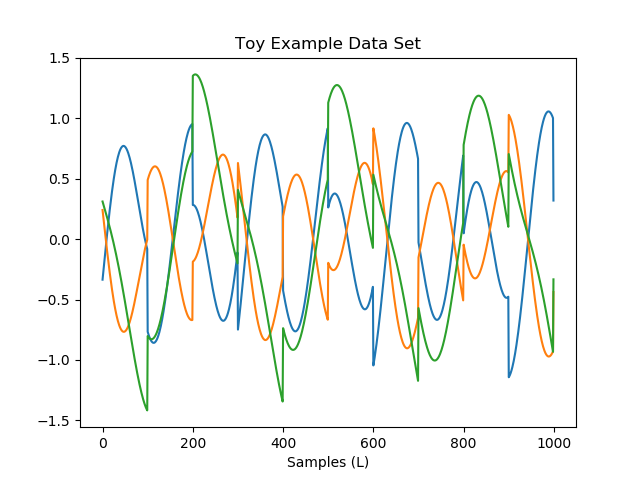
\includegraphics[scale=0.5]{figures/chapter6/Mix_Data_m3_n4_k4_L1000.png}
\label{fig:mix}
\caption{All the signal of the toy example data set for $M = 3$, $k=4$ and $L=1000$.}
\end{figure}
\noindent

\subsubsection{Autoregressive}
The second data set illustrate a more realistic data set.
The data set is constructed from different autoregressive processes: 
\begin{itemize}
\item[-] $\mathbf{x}^{t} = \mathbf{a1}^{t-1} \cdot \mathbf{x}^{t-1} + \mathbf{a1}^{t-2} \cdot \mathbf{x}^{t-2} + \mathbf{w1}_t$
\item[-] $\mathbf{x}^{t+1} = \mathbf{a2}_t \cdot \mathbf{x}_{t-1} + \mathbf{a}_t \cdot \mathbf{x}_t + \mathbf{w}_t$
\item[-] $\mathbf{x}_{t+1} = \mathbf{a}_t \cdot \mathbf{x}_{t-2} + \mathbf{a}_t \cdot \mathbf{x}_t + + \mathbf{a}_t \cdot \mathbf{x}_{t-1} \mathbf{w}_t$
\item[-] $\mathbf{x}_{t+1} = \mathbf{a}_t \cdot \mathbf{x}_t + \mathbf{a}_t \cdot \mathbf{x}_{t-3} + \mathbf{w}_t$
\end{itemize}
with $t$ being a time index defined in the interval $[0,10]$ with $L$ samples. Each of the four signal are randomly drawn and used to construct a source matrix $\mathbf{X}$ of size $k \times L$. 
With a source matrix $\mathbf{X}$ a mixing matrix $\mathbf{A}$ of size $M \times k$ is randomly generated from a Gaussian distribution and then normalised. By multiplying the source matrix and the mixing matrix the measurement matrix $\mathbf{Y}$ is achieved and this complete the toy example data set.

An illustration of the data set can be seen in figure \ref{fig:mix}. The data set is constructed for $M = 3$, $k = 4$ and $L = 1000$.
\begin{figure}[H]
\centering
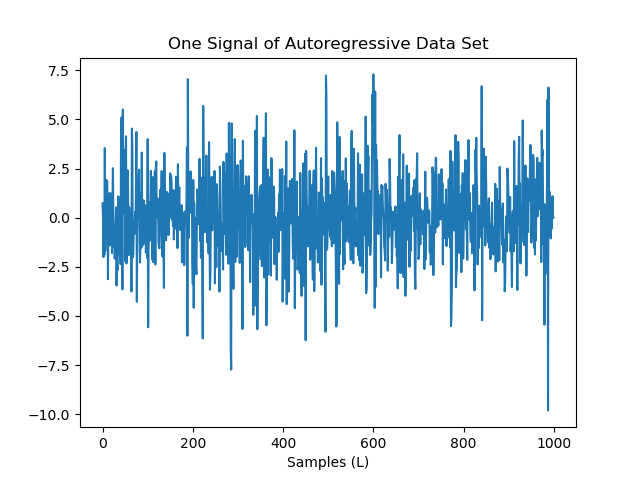
\includegraphics[scale=0.5]{figures/chapter6/AR_Data_m3_n4_k4_L1000.png}
\label{fig:mix}
\caption{All the signal of the toy example data set for $M = 3$, $k=4$ and $L=1000$.}
\end{figure}
\noindent

\subsection{Tests}

\subsubsection{Initial A in Cov-DL}

M = 8, k = 16

\begin{table}[H]
\centering
\begin{tabular}{|c|c|c|c|}
\hline 
 & A1 & A2 & A3 \\ 
\hline 
MSE & 0.70 & 0.65 & 25.98 \\ 
\hline 
\end{tabular} 
\caption{Toy Example Data Set}
\end{table}


\begin{table}[H]
\centering
\begin{tabular}{|c|c|c|c|}
\hline 
 & A1 & A2 & A3 \\ 
\hline 
MSE & 1.35 & 2.17 & 16.50 \\ 
\hline 
\end{tabular} 
\caption{AR Data Set}
\end{table}